\documentclass[conference, a4paper]{IEEEtran}
\IEEEoverridecommandlockouts
% The preceding line is only needed to identify funding in the first footnote. If that is unneeded, please comment it out.
\usepackage[T1]{fontenc}
\usepackage{cite}
\usepackage{amsmath,amssymb,amsfonts}
\usepackage{algorithmic}
\usepackage{graphicx}
\usepackage{textcomp}
\usepackage{xcolor}
\usepackage{hyperref}
\usepackage[capitalise]{cleveref}
% \usepackage{natbib}
%max package
\usepackage[colorinlistoftodos]{todonotes}
% Bibliography


\def\BibTeX{{\rm B\kern-.05em{\sc i\kern-.025em b}\kern-.08em
    T\kern-.1667em\lower.7ex\hbox{E}\kern-.125emX}}
    
\begin{document}

\title{Towards the open source electricity network modelling of the African continent\
%\thanks{Include funding agency}
}
% ORDER OF AUTHORS TO BE FINALISED LATER - THIS IS JUST TO SEE HOW MUCH SPACE IT TAKES :)
\author{\IEEEauthorblockN{Desen Kirli}
\IEEEauthorblockA{\textit{Institute for Energy Systems} \\
\textit{University of Edinburgh}\\
Edinburgh, Scotland, United Kingdom \\
\href{mailto:desen.kirli@ed.ac.uk}{desen.kirli@ed.ac.uk} \\
\url{https://orcid.org/0000-0001-7596-0944}}
\and
\IEEEauthorblockN{Johannes Hampp}
\IEEEauthorblockA{\textit{Center for International Development} \\
\textit{and Environmental Research} \\
\textit{Justus-Liebig-University Giessen}\\
Giessen, Germany \\
\href{mailto:johannes.hampp@zeu.uni-giessen.de}{johannes.hampp@zeu.uni-giessen.de}\\
\url{https://orcid.org/0000-0002-1776-116X}}
\and
\IEEEauthorblockN{Koen van Greevenbroek}
\IEEEauthorblockA{\textit{Department of Computer Science} \\
\textit{UiT The Arctic University of Norway}\\
Tromsø, Norway \\
\href{mailto:koen.v.greevenbroek@uit.no}{koen.v.greevenbroek@uit.no} \\
\url{https://orcid.org/0000-0002-6105-2846}}
\and
\IEEEauthorblockN{Rebecca Grant}
\IEEEauthorblockA{\textit{Institute} \\
\textit{University of Edinburgh}\\
Edinburgh, Scotland, United Kingdom \\
\href{mailto:xxxx@ed.ac.uk}{xxxx@ed.ac.uk} \\
\url{https://orcid.org/}}
\and
\IEEEauthorblockN{Matin Mahmood}
\IEEEauthorblockA{\textit{Institute for Energy Systems} \\
\textit{University of Edinburgh}\\
Edinburgh, Scotland, United Kingdom \\
\href{mailto:xxxx@ed.ac.uk}{xxxx@ed.ac.uk} \\
\url{https://orcid.org/}}
\and
\IEEEauthorblockN{Maximillian Parzen}
\IEEEauthorblockA{\textit{Institute for Energy Systems} \\
\textit{University of Edinburgh}\\
Edinburgh, Scotland, United Kingdom \\
\href{mailto:max.parzen@sms.ed.ac.uk}{max.parzen@sms.ed.ac.uk} \\
\url{https://orcid.org/0000-0002-4390-0063}}
\and
\IEEEauthorblockN{Aristides Kiprakis}
\IEEEauthorblockA{\textit{Institute for Energy Systems} \\
\textit{University of Edinburgh}\\
Edinburgh, Scotland, United Kingdom \\
\href{mailto:kiprakis@ed.ac.uk}{kiprakis@ed.ac.uk} \\
\url{https://orcid.org/0000-0001-7596-0944}}
}

\maketitle

\begin{abstract} %250 words
Electricity network modelling and grid simulations form the key for integrating newer and cleaner technologies such as renewable energy generators and electrical cars. This paper reviews the existing modelling packages and highlights the gap in the open source (OS) modelling of the African electricity network.
Using PyPSA (i.e. an OS Power System Analysis package), the paper outlines the pathway to a fully OS module and data to increase the transparency in the African network modelling.
Simulation of smart grid technologies will reveal the strong and weak parts of the grid which would accelerate their adoption in Africa and help with the strategic planning for upgrades and policy-making.
\end{abstract}

\begin{IEEEkeywords} % at least three, put in alphebetical order
Africa, open access, open source software, electricity access, geospatial modelling, network modelling, transmission system, electricity grid
\end{IEEEkeywords}

% \section*{Paper Guidelines from AFRICON2021}

% \begin{itemize}
% \item Papers should be written in English with a maximum paper length of \textcolor{red}{six (6) printed pages} (two-column format, 10-point font) using the supplied paper template including figures without incurring any page charges. 
% \item DEADLINE: \textcolor{red}{30/04/2021}
% \item all existing AFRICON proceedings live here since '92 \href{https://ieeexplore.ieee.org/xpl/conhome/1000025/all-proceedings}{\textbf{here}}
% \end{itemize}
 

\section{Introduction}
% \todo[inline]{Koen: personally, I would replace ``OS'' by ``open source'' everywhere. It doesn't save enough space to be worth the mental overhead of this abbreviation.}
The open source (OS) models and open-modelling initiatives in Europe bridge the gap between policymaking and long-term planning performed by researchers. For developing countries including but not limited to the ones located in the African continent, it is essential to simulate long-term energy portfolio scenarios as economic viability, risk and return on investments are key for investments in electrification and integration of renewable energy sources (RES).

Even though there are existing OS models and modelling tools in literature, there is a gap in evaluating the existing work that focuses specifically on Africa which is rich in many different kinds of RES such as solar and wind.
Here, we both review the existing work and also propose a roadmap to OS energy systems modelling in Africa.

The main contributions of this paper are outlines below:
\begin{itemize}
    \item A review of the existing OS energy systems models of Africa and categorisation of the existing work into academic and non-academic initiatives.
    \item A presentation of the proposed roadmap for our modelling initiative which has a focus on integration of RES and smart grid technologies such as batteries and electric vehicles.
\end{itemize}


\section{Review of the Existing Work, Initiatives and Motivation}
In this section, firstly, we discuss the motivation for OS modelling in Africa and drivers in terms of rapid development such as interconnection projects between African countries. Secondly, the existing work is presented, reviewed and split into two categories which are academic and non-academic developments in energy systems planning for Africa.

\subsection{Motivation and existing projects for energy systems developments in Africa}
There are numerous initiatives to increase electrification and develop the resilience of the grid in Africa. One of the well-known methods for increasing resiliency is using introducing interconnection between countries such as the one between the UK and France. Despite the more complex modelling, simulation and computational costs, the advantages include higher system inertia and more stable frequency. \Cref{interconnector} (presented in Conference on Power Transmission in Africa 2019) shows the projects for interconnections between various countries in Sub-Saharan Africa.

\begin{figure}[t]
\centerline{\includegraphics[width = 0.45\textwidth]{Figures/interconnector.jpg}}
\caption{Interconnector projects in Africa [REF!].}
\label{interconnector}
\end{figure}



\subsection{Existing Non-Academic Initiatives}
\begin{itemize}
\item Southern African Power Pool \href{https://globaltransmission.info/archive.php?id=36051}{\textbf{here}}
\item EMP-A: Energy Modelling Platform Africa \href{http://www.energymodellingplatform.org/africa.html}{\textbf{here}}
\begin{itemize}
\item OS energy MOdelling SYStem (OSeMOSYS) \cite{howells-rogner-ea-2011}
\item Geo-spatial Electrification Modelling [ref!]
\end{itemize}
\item 
\item EU Energy projections for African countries \href{https://op.europa.eu/en/publication-detail/-/publication/5bfffb22-fe1d-11e9-8c1f-01aa75ed71a1/language-en}{\textbf{here}}
\item Energy	futures	modelling	for	African	cities	– selecting	a	modelling	tool for the	SAMSET	project  \href{https://media.africaportal.org/documents/14Tait-etal-energy_futures_modelling.pdf}{\textbf{here}}
\item Energy planning and modelling support in Africa \href{{https://irena.org/-/media/Files/IRENA/Planning/IRENA_Modelling_support_Africa_2020.pdf?la=en&hash=C66FD1D23605A4F5065FBA47896EC55060A85B41}}{\textbf{here}}

\item open mod - working on specifically on the african continent

\end{itemize}

\subsection{Existing Academic Work}
\todo[inline]{Desen: My vision for this section is to highlight all the work done using other models categorising them into "local use of established energy modelling tools (that have a physics-based calculations)" such as Calliope in SA and Kenya (i.e. small application area, capable tool) and "wide-area application of GIS/non-physics-informed tools" such as the implementation of OnSSET in Africa, other tools in Sub-Saharan Africa. (i.e. large application area, non-physics-informed tool). The aim is to frame the existing work and highlight the gap of using a physics-informed electricity modelling tool (i.e. PyPSA) for the whole continent. The motivation for this is covered previously as interconnection plans exist and previous experience in Europe and especially the winter black-out in Texas show the importance of interconnection and resilience of the grid}



 However, geographical Information Systems (GIS) data is increasingly being utilised to better. The integration of GIS data into demand prediction and projection in models such as OSeMOSYS~\cite{howells-rogner-ea-2011}, e.g., in~\cite{rocco-fumagalli-ea-2021}, offer new potential to better understand demand needs.  

Lighting the World: the first application of an open source, spatial electrification tool (OnSSET) on Sub-Saharan Africa
\citet{mentis-howells-ea-2017} \cite{mentis-howells-ea-2017} implemented the first use of 


\subsubsection{Least Cost Electrification Analysis}

\todo[inline]{Koen: this section is under construction!}

% Computer modelling to map potential pathways for rural electrification is widespread, especially within the Global South~\cite{bertheau-cader-ea-2016,cader-blechinger-ea-2016,alfaro-miller-2021,rocco-fumagalli-ea-2021,anwar-deshmukh-ea-2020}. Systematic reviews have sought to understand how different modelling tools, including HOMER Energy, Network Planner, and GEOSIM, calculate least cost electrification options for rural regions of Sub-Saharan Africa. Challenges exist with respect to the collection of data for input parameters such as population and electricity demand, especially for remote regions. There are additional complexities modelling decentralised options such as solar PV, diesel generation and hybrid mini-grids,  which require hourly simulations to ensure their economic and technological appropriateness to context~\cite{cader-blechinger-ea-2016}. A set of deficits relating to the use of modelling tools is identified in~\cite{cader-blechinger-ea-2016}, including: HOMER, which doesn’t consider stand-alone systems, Network Planner, which doesn’t model hydrid mini-grids and whose methodology promotes grid connection based on  proximity (regardless of topography or infrastructure), and GEOSIM, which despite incorporating constraints such as available investment and on-grid energy generation does not model solar hybrid mini-grids~\cite{cader-blechinger-ea-2016}.

Geospatial electrification analysis combines GIS analysis with least cost technology planning approaches to map least cost electrification options where electricity access is low~\cite{mentis-howells-ea-2017,trotter-cooper-ea-2019}. This has been carried out at a country level in Sub-Saharan Africa including for Nigeria~\cite{mentis-siyal-ea-2017,nerini-broad-ea-2016,mentis-welsch-ea-2015}, Ethiopia~\cite{mentis-andersson-ea-2016}, Kenya~\cite{mentis-howells-ea-2017,szabo-moner-girona-ea-2016,mentis-welsch-ea-2015}, Uganda~\cite{trotter-cooper-ea-2019}, Burkino Faso and Cote d’Ivoire~\cite{bissiri-moura-ea-2020}, in Malawi~\cite{korkovelos-khavari-ea-2019} and in Tanzania~\cite{menghwani-zerriffi-ea-2020}. The OnSSET model is especially popular as a spatial electrification analysis tool for Sub-Saharan Africa. These case studies vary with respect to parameters used, though most include desired electricity target level and quality of access, population density, local grid connection status, existing electricity infrastructures, energy resource availability and cost of energy technologies in their assessments~\cite{menghwani-zerriffi-ea-2020}. A review of energy system modelling carried out in~\cite{rocco-fumagalli-ea-2021} finds increasing trends towards OS energy modelling (e.g., OnSSET) in Sub-Saharan Africa, highlighting tendencies towards aggregation of certain nationally specific data (such as investment, policy, and production efficiencies) across Sub-Saharan Africa or regionally (e.g., in East Africa). They also draw attention to issues associated with defining and predicting electricity demand for rural regions which homogenise rural energy users as a single user group. Energy modelling requires assumptions of energy demand so as to ensure appropriate choice and sizing of electrification option. However, issues have been identified with the processes of defining rural electricity demand, with some models homogenising rural energy users as a single user group irrespective of distance from the grid and population size. However, geographical Information Systems (GIS) data is increasingly being utilised to better. The integration of GIS data into demand prediction and projection in models such as OSeMOSYS~\cite{howells-rogner-ea-2011}, e.g., in~\cite{rocco-fumagalli-ea-2021}, offer new potential to better understand demand needs.  

Agent-Based Modelling (ABM) is increasingly being applied to energy system modelling~\cite{alfaro-miller-2021,riva-colombo-2020}. It is utilised in~\cite{alfaro-miller-2021} to determine least cost options for rural electrification under scenarios of 100\% renewable energy generation. Recently, machine learning was utilised in~\cite{alova-trotter-ea-2021} to predict future electrification pathways and generation mixes in Africa. Further scope has also been identified with respect to developing energy system models for SSA which incorporate different energy storage technologies (see~\cite{musonye-davidsdottir-ea-2020}).
\begin{itemize}
\item \cite{schlott-schyska-ea-2020}. \todo[inline]{Koen: the relevance of this is questionable.}
\item \cite{phongtrakul-kongjeen-ea-2018}. \todo[inline]{Koen: Is this relevant? It doesn't seem like such an interesting paper in our context or am I missing something?}
\item OSeMOSYS~\cite{howells-rogner-ea-2011}.
\item Lighting the World: the first application of an open source, spatial electrification tool (OnSSET) on Sub-Saharan Africa~\cite{mentis-howells-ea-2017} (already talked about above. - this is a specific application)
\item \cite{menghwani-zerriffi-ea-2020} (A case study already mentioned above.)
\item Calliope~\cite{pfenninger-pickering-2018}. \emph{NOTE (Koen): Anything more specific? Could include a brief listing of currently developed open energy system models?}

\item \todo[inline]{Desen: This is what I had in mind - see South Africa and Kenya: https://www.callio.pe/model-gallery/
 (1) Calliope- Kenya: " is a five-region model of Kenya developed at Politecnico di Milano."  \url{https://github.com/SESAM-Polimi/Calliope-Kenya}
 (2) South Africa
SA-Calliope was used in a peer-reviewed paper comparing concentrating solar power (CSP) and nuclear as baseload providers in South Africa. It contains commercially licensed data and is thus not freely and publicly available~\cite{pfenninger-keirstead-2015}.}

\item Probably the most important academic existing work: TEMBA~\cite{taliotis-shivakumar-ea-2016}.
\item ``Regional Energy Supply Index (RESI): Using Open Source Data to Monitor Electricity Reliability across Sub-Saharan Africa'' - ``There is a limited body of knowledge on the power quality issues affecting micro, small and medium enterprises (MSMEs) in Africa. Power quality monitoring studies in the past have previously focused on larger formal companies and have mostly relied on surveys to collect data. The purpose of this paper is to introduce the Regional Electricity Supply Index (RESI) that seeks to standardize the collection and real-time monitoring of power supply to MSMEs across Sub-Saharan Africa'' \cite{kitetu-mbutura-2020}.

\item Review: ``Next generation interactive tool as a backbone for universal access to electricity'' - ``Energy planning in rural areas and in developing countries most often relies on the outputs of specialized analytical tools, of which only a handful have been developed. Over the years these tools have been upgraded, and the newest among them take into consideration, to a greater or lesser extent, all key determinants of energy generation and distribution. This article focuses on a “pool” of web-based geo-referencing open-source tools and highlights the extent to which each analytical tool reflects the particularities of the various determinants of energy generation and distribution. In doing so, the present work identifies aspects of the tools that need to be strengthened. Building on this information, the article further maps the suitability of each tool with regard to calculating (at a local level) the six Sustainable Development Goal indicators that are closely related to energy. This makes it possible to draw conclusions about monitoring needs in study-areas. Bringing together these two sets of findings, the article concludes with a research agenda for analytical tool development in the area of energy planning, which spills over developmental agendas'' \cite{moner-girona-puig-ea-2018}.
  
\item ``A geospatial assessment of small-scale hydropower potential in sub-saharan Africa'' - ``Sub-Saharan Africa has been at the epicenter of an ongoing global dialogue around the issue of energy poverty. More than half of the world's population without access to modern energy services lives there. It also happens to be a sub-continent with plentiful renewable energy resource potential. Hydropower is one of them, and to a large extent it remains untapped. This study focuses on the technical assessment of small-scale hydropower (0.01-10 MW) in Sub-Saharan Africa. The underlying methodology was based on open source geospatial datasets, whose combination allowed a consistent evaluation of 712,615 km of river network spanning over 44 countries. Environmental, topological, and social constraints were included in the form of constraints in the optimization algorithm. The results are presented on a country and power pool basis.'' \cite{korkovelos-mentis-ea-2018}.

\item ``PVMAPS: Software tools and data for the estimation of solar radiation and photovoltaic module performance over large geographical areas'' - ``A set of computational tools and climatic data, tentatively named PVMAPS, is presented which makes it possible to calculate solar radiation and photovoltaic system power on inclined and/or sun-tracking surfaces over large geographical areas at arbitrarily high spatial resolution. Calculations of solar radiation and photovoltaic performance are done using validated models published in the scientific literature. The software has been implemented as modules in the open-source GRASS Geographical Information System and is delivered together with scripts to perform the calculations for any geographical region in the area covered by the data. The accompanying data set includes information about elevation, horizon height, average temperatures, solar radiation (direct and diffuse components) as well as data to calculate the effects of wind and spectral variations on PV performance. The geographical extent of the data at present includes Europe, Africa and most of Asia. All tools and data are freely available at no cost. '' \cite{huld-2017}.

\item ``A geospatial approach towards defining cost-optimal electrification pathways in West Africa'' - ``West Africa holds some of the lowest electrification rates in sub-Saharan Africa with high disparities among countries and between urban and rural areas. Despite long-standing efforts to scale-up electrification levels, overall progress remains slow and highly cost-ineffective. Hence, it is crucial that electricity planning processes primarily address the questions of the complementarity between utility-scale and decentralised generation. This paper applies the Open Source Spatial Electrification Tool (OnSSET) to two ECOWAS countries – Burkina Faso and Côte d'Ivoire – with the aim of determining the optimal combination of grid-connected and off-grid systems to serve rural and urban demand by 2030, using high-resolution geospatial data. This country-wide analysis highlights the fundamental role of off-grid solar photovoltaics and wind technologies in bridging the electricity access gap, particularly in Burkina Faso. Additionally, cheaper electricity costs in Côte d'Ivoire could be taken advantage of through enhanced cross-border exchanges between the two countries.'' - 10.1016/j.energy.2020.117471
\item ``Optimal management of storage for offsetting solar power uncertainty using multistage stochastic programming'' - ``Africa has recently engaged in implementing an aggressive renewable energy integration plan. A major challenge in the deployment of renewable power is the management of excess energy. The use of battery storage has been considered as a technically attractive solution. This paper tackles this operational problem using stochastic dual dynamical programming. We present an open-source MATLAB toolbox for multistage stochastic programming which employs stochastic dual dynamic programming. We use the toolbox in order to compare the stochastic solution to a greedy policy which operates batteries without future foresight as a benchmark. We consider a case study of storage management in Burkina Faso. We quantify the benefits of the stochastic solution and test the sensitivity of our results to the optimization horizon of the stochastic program.  '' \cite{kaneda-scieur-ea-2018}.
  
\item ``Electricity infrastructure planning: Evaluating solar potential assessments for informal settlements using grass and freely available data'' - ``Informal settlements, also known as slums or shanty towns, are characterised by rapid and unstructured expansion, poorly constructed buildings, and in some cases, they are on disputed land. Such settlements often lack basic services, such as electricity. As a result, informal settlement dwellers turn to hazardous alternative sources of energy, such as illegal electricity connections and paraffin. Solar power is a clean and safe alternative. However, informal settlements are often located on undesirable land on the urban fringe where the topography may hinder the use of solar energy. The high density of dwellings could also be a hindrance. Therefore, the solar potential needs to be assessed before any implementations are planned. Solar potential assessment functionality is generally available in geographic information system (GIS) products. The nature, cost and accessibility of datasets required for the assessment vary significantly. In this paper, we evaluate the results of solar potential assessments using GRASS (Geographic Resources Analysis Support System) for a number of different datasets. The assessments were done for two informal settlements in the City of Tshwane (South Africa): Alaska, which is nestled on a hill; and Phomolong, a densely populated settlement with a rather flat topography. The results show that solar potential assessments with open source GIS software and freely available data are feasible. This eliminates the need for lengthy and bureaucratic procurement processes and reduces the financial costs of assessing solar potential for informal settlements.'' \cite{hassim-coetzee-ea-2018}

\item ``ICT for renewable energy integration into smart buildings: IoT and big data approach'' - ``SG (Smart Grids) are emerging as a very promising technology with buildings as one of its most critical components. SG are meant to leverage energy-efficiency and promote green usage via efficient renewable energy integration. SG pose inherent challenges stemming, mainly, from its inter-disciplinary nature. Besides ICT (Information and Communication Technology), SG involves two other broad disciplines: 1. Power systems and 2. Control systems. Still, ICT is the major component that manifests SG ' Smartness'. In this work, we present the architecture of a real-world smart micro-grid testbed to be deployed in a university campus. We highlight its main components with an emphasis on the ICT component. We are advocating that SG will utilize Internet of Things (IoT) to source all types of data, and thus making the whole system fall within the realm of Big Data. To handle the huge amount of data that will be collected, we advise the deployment of a private local Cloud using open source platform for HPC (High-Performance-Computing) along with Hadoop/MapReduce as the underlying data storage and processing model. We deem this project as an ideal blueprint that can be easily adopted for similar real-world smart micro-grid testbeds in Africa and around the world.'' \cite{abid-lghoul-ea-2017}.
  
\item ``Water and Energy Systems in Sustainable City Development: A Case of Sub-saharan Africa'' - ``Current urban water and energy systems are expanding while increasing attention is paid to their social, economic and environmental impacts. As a research contribution that can support real-world decision making and transitions to sustainable cities and communities, we have built a model-based and data-driven platform combining comprehensive database, agent-based simulation and resource technology network optimization for system level water and energy planning. Several use cases are demonstrated based on the Greater Accra Metropolitan Area (GAMA) city-region in Ghana, as part of the Future Cities Africa (FCA) project. The outputs depict an overall resource landscape of the studied urban area, but also provide the energy, water, and other resource balance of supply and demand from both macro and micro perspectives, which is used to propose environmental friendly and cost effective sustainable city development strategies. This work is to become a core component of the resilience.io platform as an open-source integrated systematic tool gathering social, environmental and economic data to inform urban planning, investment and policy-making for city-regions globally. '' \cite{wang-vandam-ea-2017}.
\end{itemize}

\newpage
\section{Roadmap to an Open Energy System Model for Africa}

The \emph{PyPSA meets Africa} project aims to construct the first high resolution open model of the African energy system using open data.
We are building an automated, modular and reproducible workflow based on PyPSA.

PyPSA (Python for Power System Analysis)~\cite{brown-horsch-ea-2018} an OS modelling framework with a significant number of active users.
It is used for capacity expansion and dispatch optimisation of energy systems.
A principle feature of PyPSA is relatively detailed modelling of optimal power flow in transmission networks.
This makes PyPSA well suited to large-scale models including conventional and renewable energy sources, storage technologies as well as energy carries including natural gas and hydrogen.
% PyPSA is therefore well suited for integrated models containing conventional energy sources like fossil-driven power plants, variable renewable energy sources like wind and solar, storage technologies like batteries as well as other energy carriers like natural or hydrogen gas as well as heating/cooling and mobility services.
Prominent examples of PyPSA-based models are PyPSA-Eur~\cite{PyPSAEur}, a high resolution optimisation mode of the European transmission grid, and PyPSA-Eur-Sec~\cite{PyPSAEurSec}, an extension of the former which includes sector coupling.
An example of an optimised system produced by PyPSA-Eur is shown in \autoref{EU-Map}.

% \begin{figure}[htbp]
% \centerline{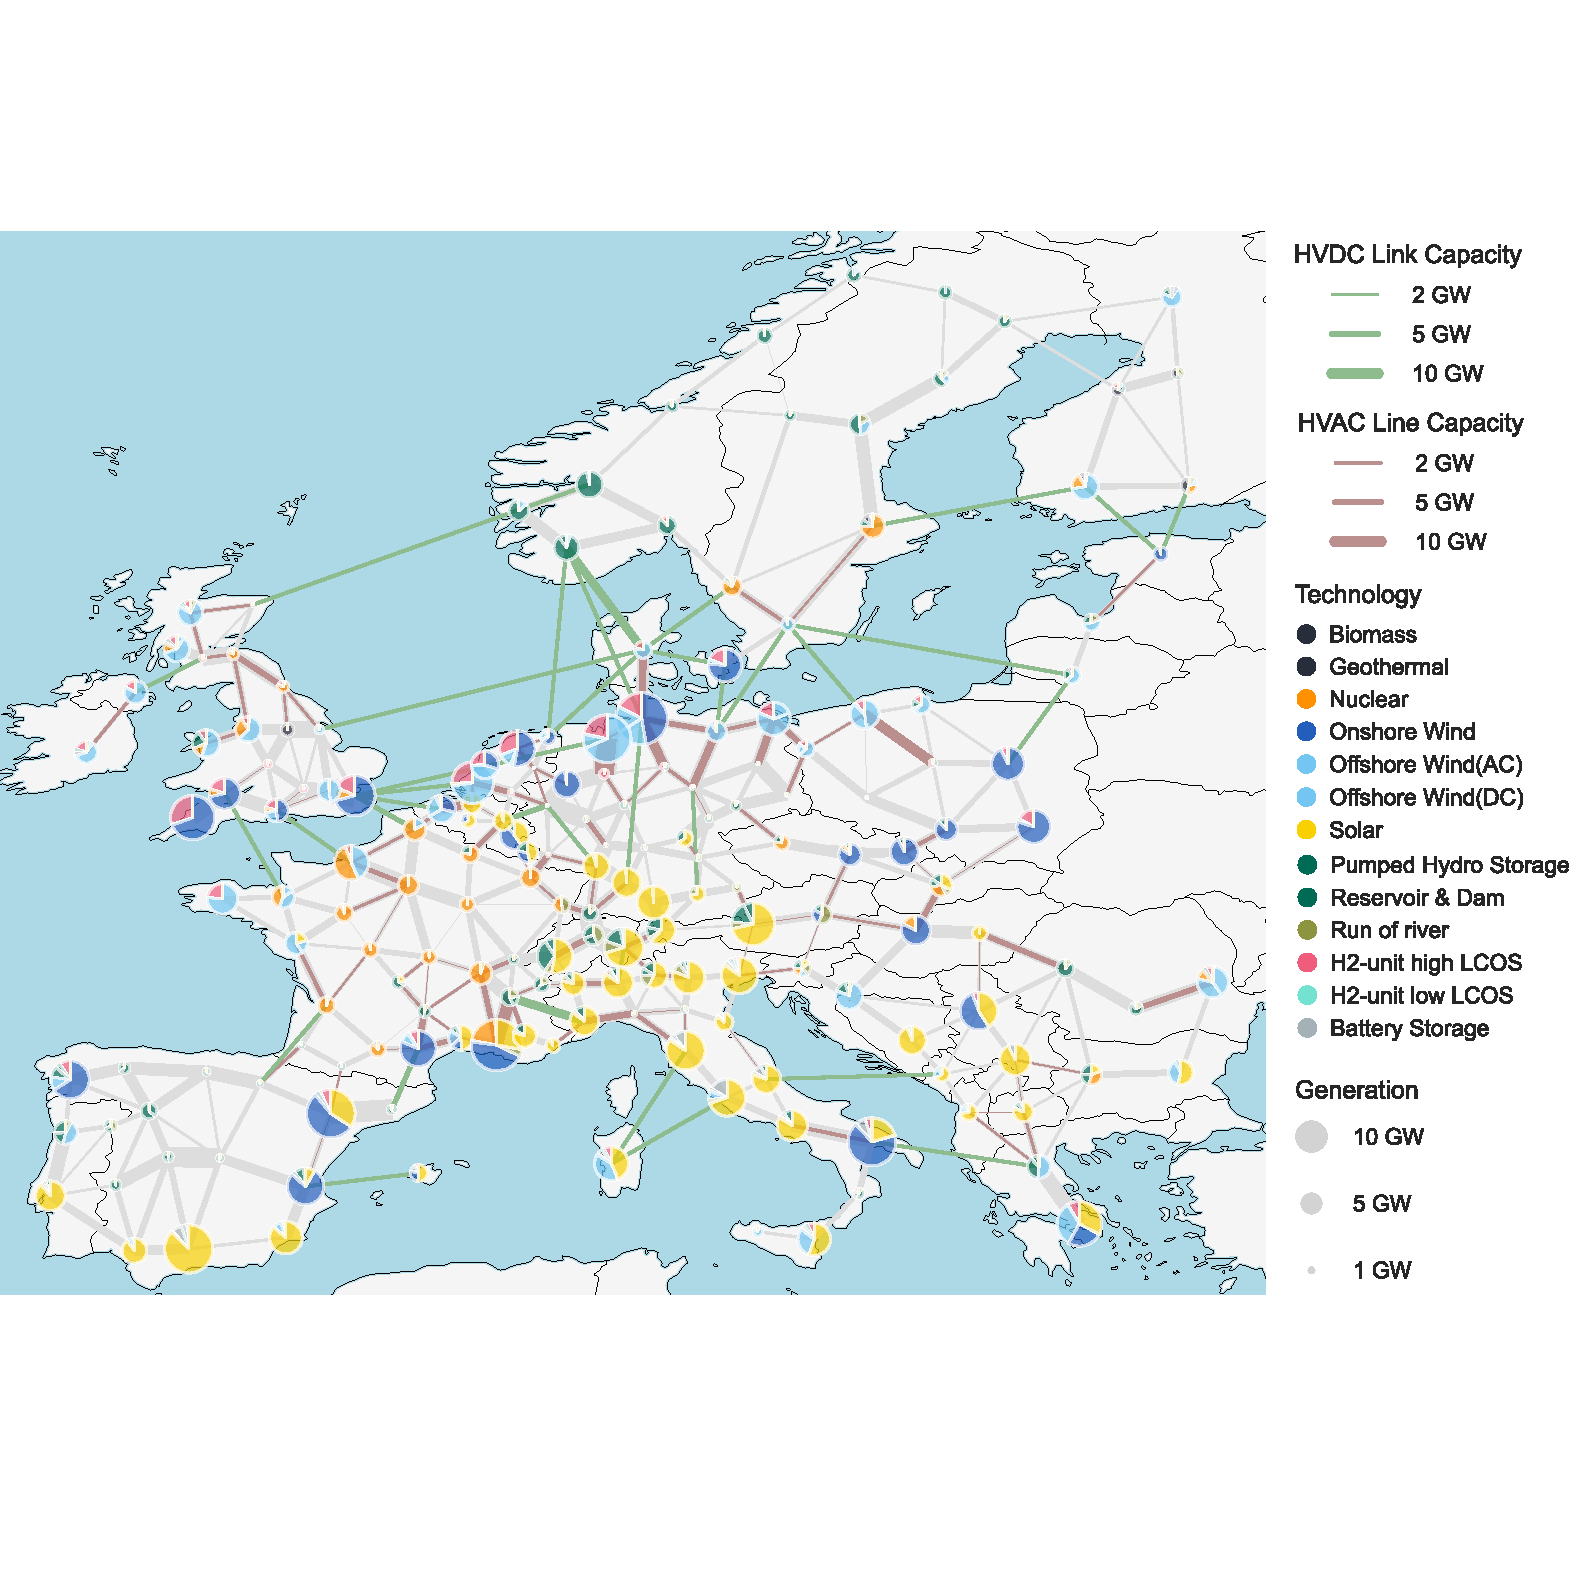
\includegraphics[width = 0.5\textwidth]{Figures/EU-generation-map2.pdf}}
% \caption{Map of planned and existing transmission lines in Africa.}
% \label{EU-Map}
% \end{figure}

%%%% VERSION TWO
\begin{figure}[htbp]
\centerline{\includegraphics[trim={0cm 0cm 0cm 3cm},clip,width = 0.5\textwidth]{Figures/EU-generation-map.pdf}}
\caption{Optimal generation, storage and network expansion in Europe under a 100\% emission reduction scenario and technology data for 2030. Light grey lines showing the existing installed network capacity~\cite{parzen-neumann-ea-2021}.}
\label{EU-Map}
\end{figure}

%%%% Africa plot with transmission lines & substations [MATIN]

\begin{figure}[htbp]
\centerline{\includegraphics[trim={4cm 8cm 4cm 8cm},clip,width = 0.5\textwidth]{Figures/africa_transmission_network_and_substations.png}}
\caption{Map of transmission lines and substations. Lines show planned and existing transmission lines over 110 kV in Africa and the MENA region. Substations show existing assets for Africa. Data available at https://energydata.info/dataset/africa-electricity-transmission-and-distribution-grid-map-2017 \& OpenStreetMap}.
\label{AfricaMApTransmission}
\end{figure}

The model being developed by PyPSA meets Africa will build on the successes of PyPSA-Eur.
It will be the first model of the African transmission grid at a high, adjustable spatial resolution.
Moreover, this is done with a modular workflow based on open data meeting the FAIR principles~\cite{wilkinson-dumontier-ea-2016}.
As a result, the model can easily be updated with improved data as it becomes available.

The project aims to work as much as possible with existing open source libraries and working code bases; see also the later subsections.
This will allow us to couple the African model with PyPSA-Eur, enabling cross-beneficial source code development, intercontinental studies, and a larger user base.
Additionally, we foresee to add the sector-coupling of PyPSA-Eur-Sec to the African model.
The ultimate goal is to create a long-term maintained and supported OS model that is useful for industry, research and policy purposes.


% further accelerate the integration of different RES technologies such as solar, wind, tidal and other marine sources and additionally smart grid objects such as batteries and electric vehicles. As shown in \cref{AfricaMApTransmission}, as an initial step to map the existing transmission lines.  This study uses the dataset made available by Onsset which ``includes planned and existing grid lines for all continental African countries and Madagascar, as well as the Middle East region. The lines range in voltage from sub-kV to 700 kV EHV lines.'' It should be noted that there is a large variation in availability of data for different countries.


The project is split into multiple work packages which are layed out in the next subsections including an outlook on the methodology planned for each work package:

\begin{enumerate}
    \item Demand modelling
    \item Conventional generator modelling
    \item Wind, solar, marine energy resource modelling
    \item Land coverage constraint modelling
    \item Network and substation modelling
    \item Data creation and validation 
\end{enumerate}

We aim to complete a working prototype of our model by end of 2021.

\subsection{Demand modelling} %%% Johannes
Electricity demand and time-series will be modelled using GEGIS (GlobalEnergyGIS).
GEGIS applies a machine learning approach based on existing electricity demand time-series data, population densities and spatially resolved income data.
This data is complemented with scenario information from the SSP (Shared Socioeconomic Pathways) and ERA5 reanalysis weather data to generate hourly resolved time-series for arbitrary regions for arbitrary years until 2050.
% \todo[inline]{I haven't checked the following sentence and can neither confirm nor deny its correctness.}
% GEGIS follows the open GIS standards of the Open Geospatial Consortium and is operated as shown in \cref{GEGIS}.

% \begin{figure}[htbp]
% \centerline{\includegraphics[width = 0.45\textwidth]{Figures/GeGIS.png}}
% \caption{A screenshot from GEGIS [REF!].}
% \todo[inline]{Where is this figure from? I have never seen a GUI for GEGIS.}
% \label{GEGIS}
% \end{figure}

\subsection{Conventional generator modelling} %%% Koen
Power plant data is available through the Global Power Plant Database~\cite{globalenergyobservatory-google-ea-2018}, which as regarded as one of the principle open global databases.
Commercial power plant databases have historically dominated in policy and research, but in recent years open databases are closing the gap.
For conventional generation (coal, natural gas, oil, hydro), the Global Power Plant Database has a coverage of 80--100\% (depending on the category) in terms of installed capacity, as compared to state-of-the-art commercial sources~\cite{byers-friedrich-ea-2019}.

Moreover, the database can be integrated with PyPSA using the `powerplantmatching' tool~\cite{gotzens-heinrichs-ea-2019}.
Using the powerplantmatching package makes it easy to integrate other power plant databases, and matches power plants between the various databases being used.
As such, our model can incorporate new and improved datasets as they become available without much effort.

\subsection{RES generator modelling} %%% Johannes
RES (Renewable Energy Sources) will likely be the cornerstone of most future energy systems.
For this project spatially resolved potentials and hourly resolved time-series for energy generation from wind, solar and ocean sources will be modelled using established and updated methodologies with the Python package \emph{atlite}\footnote{\url{https://github.com/PyPSA/atlite}}.
%TODO: add a reference for atlite. See https://github.com/openjournals/joss-reviews/issues/3204 for the issue at JOSS.
% Unfortunately, it looks the paper is not going to go into preprint before our submission deadline. The URL should do for now, and hopefully we can cite it in the final version of this paper.
Currently atlite supports wind turbines and photovoltaic as energy sources and uses world-wide available reanalysis data from the ERA5 complemented with irradiation data from SARAH2.
With this project the variety of energy sources is to be expanded to include concentrated solar power (CSP) and ocean energy sources like wave or tidal energy generators.

\subsection{Land coverage constraint modelling}
Land use and protected areas constrain the eligible areas for RES deployment.
Determining land constraints and considering land use for Similarly, any constraints on the surface will be modelled using Atlite.
\begin{itemize}
\item water depth we can include/exclude based on the GEBCO bathymetric dataset. Also used in PyPSA-EUR
	land usage/coverage/protected areas (tool): 
\item Can be exlucded using atlite. Severin Rydberg created GLAES for this purpose a few years ago but that tool is no longer maintained so Fabian Hofmann from the atlite team included that functionality into atlite recently.
	
\item land usage/coverage/protected areas (data): This is were it becomes tricky.
\item  Maybe global corine is suitable for land usage. Protected areas would still need to be included somehow. Potentially also population density (were again I know datasets exist but I do not know how applicable they are)
\end{itemize}


% Ok, here are just my thoughts, can someone else assist with selection/formulation?
% * I don't know which data set we can use for Land coverage and protected areas
% * Data sets I know of are limited to Europe, NA, Asia
% * Maybe the Corine dataset is available for Africa/ww and would provide land usage data 
% * In addition we would need a data set for protected areas. I have no idea what do use here
% * Niclas Mattsson used with GEGIS also some datasets and he managed world-wide coverage. Maybe we find our answer there already?
% * Yes, modelling with Atlite should be possible

\subsection{Network and substation modelling} 
The network topology for Africa will mainly be extracted from a dataset compiled by the World Bank Group~\cite{arderne-2017}, which is based on a number of different sources. The dataset includes 1818 inputs for transmission lines (above 110 kV), the total length is 4204 km. Similar to PyPSA-Eur\cite{PyPSAEur}, the mapped data will be enriched by typical physical parameters such as length dependent resistance and reactance, current thermal level and apparent power limit.

The substation geolocation with voltage level will be extracted from Open Street Maps (OSM). To be computable on typical 16GB RAM computers, a relatively new efficient OSM extraction package `esy-osmfilter'~\cite{pluta-lunsdorf-2020} will be applied that is four times faster than the common alternative, OSMOSIS~\cite{henderson-2020}. Initial results from the OSM extraction process (see result in \cref{AfricaMApTransmission}) show 2721 transmission substation data points for Africa.

As for PyPSA-Eur, the country shapes and bus location will be used to split areas into Voronoi cells which are assumed to be connected to low voltage networks. Each of the Voronoi cell contains information on existing power plant capacities, renewable resource potential timeseries, as well as demand timeseries at the substation location. The spatial model resolution can be changed by aggregating the cells by k-means clustering.

\subsection{Data creation and validation}

The amount of data on energy assets might vary per country (see \cref{AfricaMApTransmission}), reducing the usefulness and accuracy of energy system models. The missing data can be either added by energy authorities sharing data or by satellite imaginary asset recognition techniques. From experience in Europe, not even official data provided from large association such as the European Network of Transmission System Operator (ENTSO-E) are not fully reliable and might take some time to be updated\cite{gotzens-heinrichs-ea-2019,PyPSAEur}. Therefore, to validate existing and new authority energy assets data, and to add new data, machine learning offers unique opportunities. 

Machine Learning (ML) techniques will be used to create missing data and increase human validation speed by at least 33-fold compared to pure human mapping strategies~\cite{developmentseed-2018}. ML approaches should not be seen in near future to replace a human validation step as the accuracy is not satisfactory. However, ML approaches are an ideal complement to current mapping techniques and can speed up the human validation process, for instance, by providing only images that are highly likely to contain the specific energy asset. ML techniques were applied to recognise from satellite imaginary high voltage lines, substations~\cite{developmentseed-2018}, solar PV \cite{dehoog-maetschke-ea-2020} and wind turbines~\cite{zhou-irvin-ea-2019}.

\todo[inline]{Add. Example of what is possible with ML. Detect between different assets. I.e. high and low voltage assets, add physical parameters and check the age of assets (by assessing satellite data over multiple years) - Max}


The 'PyPSA meets Africa' project will focus first to create validated substation and high voltage line datasets. These datasets will be made publicly available in line with the OS modelling goal. The work should be extended on other energy assets in future.

\section{Conclusions}
In this paper, we discussed the importance of OS energy systems modelling in the African continent. The existing work in terms of both academic literature, technical reports (e.g. by United Nations) and grass roots initiatives were reviewed. Lastly, we also presented our proposed roadmap to open energy modelling and data sharing in Africa which is aimed to have a wider audience with further integrated technologies such as marine energy and grid-scale batteries scheduled to increase the resiliency of the African grid \cite{}. This is expected to accelerate the simulation and hence, later integration of renewable energy technologies.

\section*{Acknowledgments}
EPRSC Doctoral Training Partnership (EP/R513209/1) and the EPSRC Centre for Energy System Integration (EP/P001173/1) are acknowledged for their support.
All funding bodies and everyone who helped improve the paper but did not contribute to the writing/analysis/etc.


% \printbibliography

\bibliographystyle{IEEEtran}
\todo[inline]{Papers  that  have  not  been  published,even  if  they  have  been  submitted  for  publication,  should  becited as “unpublished” [4]. Papers that have been accepted forpublication should be cited as “in press” [5]}
\bibliography{bibliography}

\end{document}


% \begin{thebibliography}{00}
% \bibitem{b1} G. Eason, B. Noble, and I. N. Sneddon, ``On certain integrals of Lipschitz-Hankel type involving products of Bessel functions,'' Phil. Trans. Roy. Soc. London, vol. A247, pp. 529--551, April 1955.
% \bibitem{b2} J. Clerk Maxwell, A Treatise on Electricity and Magnetism, 3rd ed., vol. 2. Oxford: Clarendon, 1892, pp.68--73.
% \bibitem{b3} I. S. Jacobs and C. P. Bean, ``Fine particles, thin films and exchange anisotropy,'' in Magnetism, vol. III, G. T. Rado and H. Suhl, Eds. New York: Academic, 1963, pp. 271--350.
% \bibitem{b4} K. Elissa, ``Title of paper if known,'' unpublished.
% \bibitem{b5} R. Nicole, ``Title of paper with only first word capitalized,'' J. Name Stand. Abbrev., in press.
% \bibitem{b6} Y. Yorozu, M. Hirano, K. Oka, and Y. Tagawa, ``Electron spectroscopy studies on magneto-optical media and plastic substrate interface,'' IEEE Transl. J. Magn. Japan, vol. 2, pp. 740--741, August 1987 [Digests 9th Annual Conf. Magnetics Japan, p. 301, 1982].
% \bibitem{b7} M. Young, The Technical Writer's Handbook. Mill Valley, CA: University Science, 1989.
% \end{thebibliography}

% \section{Prepare Your Paper Before Styling}
% Before you begin to format your paper, first write and save the content as a 
% separate text file. Complete all content and organizational editing before 
% formatting. Please note sections \ref{AA}--\ref{SCM} below for more information on 
% proofreading, spelling and grammar.

% Keep your text and graphic files separate until after the text has been 
% formatted and styled. Do not number text heads---{\LaTeX} will do that 
% for you.

% \subsection{Abbreviations and Acronyms}\label{AA}
% Define abbreviations and acronyms the first time they are used in the text, 
% even after they have been defined in the abstract. Abbreviations such as 
% IEEE, SI, MKS, CGS, ac, dc, and rms do not have to be defined. Do not use 
% abbreviations in the title or heads unless they are unavoidable.

% \subsection{Units}
% \begin{itemize}
% \item Use either SI (MKS) or CGS as primary units. (SI units are encouraged.) English units may be used as secondary units (in parentheses). An exception would be the use of English units as identifiers in trade, such as ``3.5-inch disk drive''.
% \item Avoid combining SI and CGS units, such as current in amperes and magnetic field in oersteds. This often leads to confusion because equations do not balance dimensionally. If you must use mixed units, clearly state the units for each quantity that you use in an equation.
% \item Do not mix complete spellings and abbreviations of units: ``Wb/m\textsuperscript{2}'' or ``webers per square meter'', not ``webers/m\textsuperscript{2}''. Spell out units when they appear in text: ``. . . a few henries'', not ``. . . a few H''.
% \item Use a zero before decimal points: ``0.25'', not ``.25''. Use ``cm\textsuperscript{3}'', not ``cc''.)
% \end{itemize}

% \subsection{Equations}
% Number equations consecutively. To make your 
% equations more compact, you may use the solidus (~/~), the exp function, or 
% appropriate exponents. Italicize Roman symbols for quantities and variables, 
% but not Greek symbols. Use a long dash rather than a hyphen for a minus 
% sign. Punctuate equations with commas or periods when they are part of a 
% sentence, as in:
% \begin{equation}
% a+b=\gamma\label{eq}
% \end{equation}

% Be sure that the 
% symbols in your equation have been defined before or immediately following 
% the equation. Use ``\eqref{eq}'', not ``Eq.~\eqref{eq}'' or ``equation \eqref{eq}'', except at 
% the beginning of a sentence: ``Equation \eqref{eq} is . . .''

% \subsection{\LaTeX-Specific Advice}

% Please use ``soft'' (e.g., \verb|\eqref{Eq}|) cross references instead
% of ``hard'' references (e.g., \verb|(1)|). That will make it possible
% to combine sections, add equations, or change the order of figures or
% citations without having to go through the file line by line.

% Please don't use the \verb|{eqnarray}| equation environment. Use
% \verb|{align}| or \verb|{IEEEeqnarray}| instead. The \verb|{eqnarray}|
% environment leaves unsightly spaces around relation symbols.

% Please note that the \verb|{subequations}| environment in {\LaTeX}
% will increment the main equation counter even when there are no
% equation numbers displayed. If you forget that, you might write an
% article in which the equation numbers skip from (17) to (20), causing
% the copy editors to wonder if you've discovered a new method of
% counting.

% {\BibTeX} does not work by magic. It doesn't get the bibliographic
% data from thin air but from .bib files. If you use {\BibTeX} to produce a
% bibliography you must send the .bib files. 

% {\LaTeX} can't read your mind. If you assign the same label to a
% subsubsection and a table, you might find that Table I has been cross
% referenced as Table IV-B3. 

% {\LaTeX} does not have precognitive abilities. If you put a
% \verb|\label| command before the command that updates the counter it's
% supposed to be using, the label will pick up the last counter to be
% cross referenced instead. In particular, a \verb|\label| command
% should not go before the caption of a figure or a table.

% Do not use \verb|\nonumber| inside the \verb|{array}| environment. It
% will not stop equation numbers inside \verb|{array}| (there won't be
% any anyway) and it might stop a wanted equation number in the
% surrounding equation.

% \subsection{Some Common Mistakes}\label{SCM}
% \begin{itemize}
% \item The word ``data'' is plural, not singular.
% \item The subscript for the permeability of vacuum $\mu_{0}$, and other common scientific constants, is zero with subscript formatting, not a lowercase letter ``o''.
% \item In American English, commas, semicolons, periods, question and exclamation marks are located within quotation marks only when a complete thought or name is cited, such as a title or full quotation. When quotation marks are used, instead of a bold or italic typeface, to highlight a word or phrase, punctuation should appear outside of the quotation marks. A parenthetical phrase or statement at the end of a sentence is punctuated outside of the closing parenthesis (like this). (A parenthetical sentence is punctuated within the parentheses.)
% \item A graph within a graph is an ``inset'', not an ``insert''. The word alternatively is preferred to the word ``alternately'' (unless you really mean something that alternates).
% \item Do not use the word ``essentially'' to mean ``approximately'' or ``effectively''.
% \item In your paper title, if the words ``that uses'' can accurately replace the word ``using'', capitalize the ``u''; if not, keep using lower-cased.
% \item Be aware of the different meanings of the homophones ``affect'' and ``effect'', ``complement'' and ``compliment'', ``discreet'' and ``discrete'', ``principal'' and ``principle''.
% \item Do not confuse ``imply'' and ``infer''.
% \item The prefix ``non'' is not a word; it should be joined to the word it modifies, usually without a hyphen.
% \item There is no period after the ``et'' in the Latin abbreviation ``et al.''.
% \item The abbreviation ``i.e.'' means ``that is'', and the abbreviation ``e.g.'' means ``for example''.
% \end{itemize}
% An excellent style manual for science writers is \cite{b7}.

% \subsection{Authors and Affiliations}
% \textbf{The class file is designed for, but not limited to, six authors.} A 
% minimum of one author is required for all conference articles. Author names 
% should be listed starting from left to right and then moving down to the 
% next line. This is the author sequence that will be used in future citations 
% and by indexing services. Names should not be listed in columns nor group by 
% affiliation. Please keep your affiliations as succinct as possible (for 
% example, do not differentiate among departments of the same organization).

% \subsection{Identify the Headings}
% Headings, or heads, are organizational devices that guide the reader through 
% your paper. There are two types: component heads and text heads.

% Component heads identify the different components of your paper and are not 
% topically subordinate to each other. Examples include Acknowledgments and 
% References and, for these, the correct style to use is ``Heading 5''. Use 
% ``figure caption'' for your Figure captions, and ``table head'' for your 
% table title. Run-in heads, such as ``Abstract'', will require you to apply a 
% style (in this case, italic) in addition to the style provided by the drop 
% down menu to differentiate the head from the text.

% Text heads organize the topics on a relational, hierarchical basis. For 
% example, the paper title is the primary text head because all subsequent 
% material relates and elaborates on this one topic. If there are two or more 
% sub-topics, the next level head (uppercase Roman numerals) should be used 
% and, conversely, if there are not at least two sub-topics, then no subheads 
% should be introduced.

% \subsection{Figures and Tables}
% \paragraph{Positioning Figures and Tables} Place figures and tables at the top and 
% bottom of columns. Avoid placing them in the middle of columns. Large 
% figures and tables may span across both columns. Figure captions should be 
% below the figures; table heads should appear above the tables. Insert 
% figures and tables after they are cited in the text. Use the abbreviation 
% ``Fig.~\ref{fig}'', even at the beginning of a sentence.

% \begin{table}[htbp]
% \caption{Table Type Styles}
% \begin{center}
% \begin{tabular}{|c|c|c|c|}
% \hline
% \textbf{Table}&\multicolumn{3}{|c|}{\textbf{Table Column Head}} \\
% \cline{2-4} 
% \textbf{Head} & \textbf{\textit{Table column subhead}}& \textbf{\textit{Subhead}}& \textbf{\textit{Subhead}} \\
% \hline
% copy& More table copy$^{\mathrm{a}}$& &  \\
% \hline
% \multicolumn{4}{l}{$^{\mathrm{a}}$Sample of a Table footnote.}
% \end{tabular}
% \label{tab1}
% \end{center}
% \end{table}

% \begin{figure}[htbp]
% \centerline{\includegraphics{fig1.png}}
% \caption{Example of a figure caption.}
% \label{fig}
% \end{figure}

% Figure Labels: Use 8 point Times New Roman for Figure labels. Use words 
% rather than symbols or abbreviations when writing Figure axis labels to 
% avoid confusing the reader. As an example, write the quantity 
% ``Magnetization'', or ``Magnetization, M'', not just ``M''. If including 
% units in the label, present them within parentheses. Do not label axes only 
% with units. In the example, write ``Magnetization (A/m)'' or ``Magnetization 
% \{A[m(1)]\}'', not just ``A/m''. Do not label axes with a ratio of 
% quantities and units. For example, write ``Temperature (K)'', not 
% ``Temperature/K''.